\documentclass{article}
\usepackage[margin=0.75in]{geometry}
\usepackage{tikz}
\usetikzlibrary{positioning,arrows.meta,calc,shapes.geometric,trees}
\usepackage{tcolorbox}
\usepackage{xcolor}
\usepackage{amssymb}

\newcommand{\benchmark}{ChessChain}

\begin{document}

\begin{figure}[t]
    \centering

    % Chess problem - Version 2: Compact tree structure
    \begin{tcolorbox}[
        title=\textbf{Chess: Minimax Search} \hfill {\small\colorbox{orange!20}{Easy} \quad 6 orderings},
        colframe=orange!70!black,
        colback=orange!3,
        boxrule=0.8pt,
        width=\textwidth
    ]
    \small

    \textbf{Dependency graph:}
    \begin{center}
    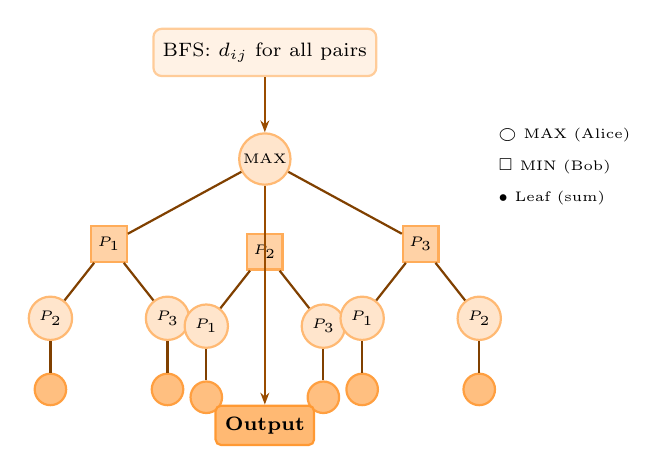
\begin{tikzpicture}[
        node distance=0.5cm and 0.6cm,
        every node/.style={font=\scriptsize},
        bfsbox/.style={draw, rounded corners=3pt, fill=orange!10, minimum width=2.2cm, minimum height=0.6cm, thick, draw=orange!40, font=\scriptsize},
        maxnode/.style={draw, circle, fill=orange!20, minimum size=0.55cm, thick, draw=orange!55, inner sep=1pt},
        minnode/.style={draw, rectangle, fill=orange!35, minimum size=0.45cm, thick, draw=orange!65, inner sep=1pt},
        leafnode/.style={draw, circle, fill=orange!50, minimum size=0.4cm, thick, draw=orange!75, inner sep=0pt, font=\tiny},
        outputnode/.style={draw, rounded corners=2pt, fill=orange!55, minimum width=1.0cm, minimum height=0.5cm, thick, draw=orange!80, font=\scriptsize\bfseries},
        arrow/.style={-{Stealth[length=1.5mm]}, thick, orange!60!black},
        treearrow/.style={-, thick, orange!50!black}
    ]
        % BFS computation box
        \node[bfsbox] (bfs) {BFS: $d_{ij}$ for all pairs};

        % Root MAX node (Alice's first choice)
        \node[maxnode, below=0.7cm of bfs] (root) {\tiny MAX};

        % First level - Alice chooses first pawn (3 choices)
        \node[minnode, below left=0.6cm and 1.5cm of root] (m1) {\tiny$P_1$};
        \node[minnode, below=0.6cm of root] (m2) {\tiny$P_2$};
        \node[minnode, below right=0.6cm and 1.5cm of root] (m3) {\tiny$P_3$};

        % Second level - Bob chooses second pawn (2 choices each)
        \node[maxnode, below left=0.5cm and 0.3cm of m1] (m1a) {\tiny$P_2$};
        \node[maxnode, below right=0.5cm and 0.3cm of m1] (m1b) {\tiny$P_3$};
        \node[maxnode, below left=0.5cm and 0.3cm of m2] (m2a) {\tiny$P_1$};
        \node[maxnode, below right=0.5cm and 0.3cm of m2] (m2b) {\tiny$P_3$};
        \node[maxnode, below left=0.5cm and 0.3cm of m3] (m3a) {\tiny$P_1$};
        \node[maxnode, below right=0.5cm and 0.3cm of m3] (m3b) {\tiny$P_2$};

        % Leaf nodes - final pawn captured (values computed)
        \node[leafnode, below=0.4cm of m1a] (l1) {};
        \node[leafnode, below=0.4cm of m1b] (l2) {};
        \node[leafnode, below=0.4cm of m2a] (l3) {};
        \node[leafnode, below=0.4cm of m2b] (l4) {};
        \node[leafnode, below=0.4cm of m3a] (l5) {};
        \node[leafnode, below=0.4cm of m3b] (l6) {};

        % Output node
        \node[outputnode, below=0.7cm of m2, yshift=-1.0cm] (out) {\textbf{Output}};

        % Tree edges
        \draw[treearrow] (root) -- (m1);
        \draw[treearrow] (root) -- (m2);
        \draw[treearrow] (root) -- (m3);

        \draw[treearrow] (m1) -- (m1a);
        \draw[treearrow] (m1) -- (m1b);
        \draw[treearrow] (m2) -- (m2a);
        \draw[treearrow] (m2) -- (m2b);
        \draw[treearrow] (m3) -- (m3a);
        \draw[treearrow] (m3) -- (m3b);

        \draw[treearrow] (m1a) -- (l1);
        \draw[treearrow] (m1b) -- (l2);
        \draw[treearrow] (m2a) -- (l3);
        \draw[treearrow] (m2b) -- (l4);
        \draw[treearrow] (m3a) -- (l5);
        \draw[treearrow] (m3b) -- (l6);

        % Arrow from BFS to root
        \draw[arrow] (bfs) -- (root);

        % Arrow from tree to output
        \draw[arrow] (root) to[out=-90, in=90] (out);

        % Legend
        \node[font=\tiny, anchor=west] at ([xshift=2.5cm, yshift=0.3cm]root.east) {$\bigcirc$ MAX (Alice)};
        \node[font=\tiny, anchor=west] at ([xshift=2.5cm, yshift=-0.1cm]root.east) {$\square$ MIN (Bob)};
        \node[font=\tiny, anchor=west] at ([xshift=2.5cm, yshift=-0.5cm]root.east) {$\bullet$ Leaf (sum)};

    \end{tikzpicture}
    \end{center}

    \vspace{-0.1cm}
    \begin{tabular}{@{}p{0.55\textwidth}p{0.42\textwidth}@{}}
    \textit{Structure:} Game tree with $3! = 6$ leaves representing all pawn capture orderings. Each leaf sums the BFS distances along its path. &
    \textit{Evaluation:} Minimax backpropagation finds optimal play value. \\
    \end{tabular}

    \vspace{0.2cm}
    \hfill \textbf{Answer:} [Redacted]
    \end{tcolorbox}

    \caption{\textbf{Chess dependency graph (compact):} BFS precomputes all pairwise distances, then minimax searches the game tree. Circles = MAX nodes (Alice maximizes), squares = MIN nodes (Bob minimizes), filled circles = leaf evaluations.}
\end{figure}

\end{document}
